\documentclass[11pt,a4paper]{article}

\usepackage[utf8]{inputenc}
\usepackage[T1]{fontenc}
\usepackage[italian]{babel} % su Overleaf funziona; se compilate in locale serve texlive-lang-italian
\usepackage[margin=2.5cm]{geometry}
\usepackage{graphicx}
\usepackage{booktabs}
\usepackage{amsmath}
\usepackage{hyperref}
\usepackage{float}

\title{Previsione dell'insolvenza creditizia\\
\large Progetto del corso di Introduzione al Pensiero Computazionale e alla Data Science\\
a.a. 2025/26}
\author{Gruppo N.~1\\[2pt]
\small Cota Miriam (1216760) \and \small Monopoli Alessandro (1232093) \and \small Ponissi Giuliana (1216083)}
\date{Luglio 2026}

\begin{document}

\maketitle

\begin{abstract}
Questo lavoro analizza il dataset \emph{Default of Credit Card Clients} (30.000 clienti di carte di credito taiwanesi) con l'obiettivo di prevedere l'insolvenza sul pagamento del mese successivo. Dopo una fase di comprensione e pulizia dei dati e un'analisi esplorativa, confrontiamo tre modelli di classificazione: regressione logistica, $k$-Nearest Neighbors e Random Forest. Alla soglia di decisione standard la Random Forest ottiene i risultati migliori (accuracy 0,813; F1 sulla classe insolvente 0,464), ma tutti i modelli mostrano recall modesti sulla classe minoritaria, conseguenza dello sbilanciamento delle classi. Una serie di esperimenti di robustezza mostra che i risultati sono stabili rispetto alla proporzione dello split e al numero di alberi, mentre la calibrazione della soglia di decisione incide sui risultati pi\`u della scelta dell'algoritmo: abbassando la soglia a 0,3, la regressione logistica raggiunge F1 0,503. Lo storico dei ritardi di pagamento, e in particolare lo stato del pagamento pi\`u recente, risulta di gran lunga il predittore pi\`u importante. Tutto il materiale del progetto \`e disponibile nel repository GitHub:\\
\url{https://github.com/etooooooooo/Gruppo-1--Data-Science}.
\end{abstract}

\section{Introduzione}

La previsione dell'insolvenza creditizia \`e un problema centrale per gli istituti finanziari: identificare in anticipo i clienti a rischio consente di limitare le perdite e di gestire meglio il credito concesso. Si tratta di un classico problema di \emph{classificazione binaria}: a partire dalle caratteristiche di un cliente, il modello deve prevedere se nel mese successivo il cliente sar\`a insolvente (classe 1) oppure no (classe 0).

L'obiettivo del progetto non \`e solo addestrare un modello, ma sviluppare un'analisi completa e riproducibile: comprensione del dataset e dei suoi limiti, analisi esplorativa guidata da domande e ipotesi, confronto fra modelli di natura diversa, verifica della robustezza dei risultati rispetto alle principali scelte di modellazione e interpretazione critica dei risultati. Il lavoro \`e stato svolto con Python e le librerie presentate durante il corso (\texttt{pandas}, \texttt{seaborn}, \texttt{matplotlib}, \texttt{scikit-learn}), versionato su GitHub e documentato in un notebook eseguibile.

Nel corso del progetto \`e stato utilizzato un assistente LLM (Claude) per la convalida del codice, il miglioramento della resa grafica e la risoluzione di errori, come documentato nel notebook; tutto il codice \`e stato rivisto e compreso dai membri del gruppo.

\section{Dataset}

Il dataset \emph{Default of Credit Card Clients}~\cite{yeh2009} contiene 30.000 record relativi a clienti di carte di credito taiwanesi, osservati da aprile a settembre 2005. Ogni record comprende 23 variabili esplicative: il credito concesso (\texttt{LIMIT\_BAL}), quattro variabili demografiche (sesso, istruzione, stato civile, et\`a), sei variabili di stato dei pagamenti mensili (\texttt{PAY\_0}--\texttt{PAY\_6}, dove $-1$ indica pagamento puntuale e i valori $\geq 1$ i mesi di ritardo), sei importi di estratto conto (\texttt{BILL\_AMT1}--\texttt{BILL\_AMT6}) e sei importi pagati (\texttt{PAY\_AMT1}--\texttt{PAY\_AMT6}). La variabile target \`e binaria: 1 se il cliente \`e risultato insolvente il mese successivo, 0 altrimenti.

\subsection{Qualit\`a dei dati e criticit\`a}

Il dataset non presenta valori mancanti n\'e identificativi duplicati. L'analisi ha per\`o evidenziato tre criticit\`a rilevanti, che abbiamo documentato e gestito.

\paragraph{Sbilanciamento delle classi.} Solo il 22,1\% dei clienti \`e insolvente. Un classificatore banale che predice sempre la classe maggioritaria otterrebbe quindi un'accuracy del 77,9\%: questo valore costituisce la \emph{baseline} di riferimento e impone di valutare i modelli anche con precision, recall e F1-score sulla classe minoritaria.

\paragraph{Valori non documentati.} Le variabili \texttt{EDUCATION} (valori 0, 5, 6, in 468 casi) e \texttt{MARRIAGE} (valore 0, in 54 casi) contengono codici assenti dalla documentazione. Li abbiamo accorpati nella categoria ``altro''. Anche le variabili \texttt{PAY\_*} contengono i valori non documentati $-2$ e 0, che coprono la maggioranza delle osservazioni: confrontandoli con gli importi fatturati, l'interpretazione pi\`u coerente \`e che $-2$ indichi assenza di consumi nel mese e 0 l'uso del credito \emph{revolving} (pagamento minimo). Abbiamo mantenuto tali valori trattando \texttt{PAY\_*} come scala ordinale di gravit\`a del ritardo.

\paragraph{Ridondanza e outlier.} Le sei variabili \texttt{BILL\_AMT} sono fortemente correlate fra loro ($r$ fra 0,80 e 0,95), con conseguente multicollinearit\`a; gli importi presentano inoltre code molto lunghe (es. \texttt{PAY\_AMT1}: mediana 2.100 NT\$, massimo 873.552 NT\$) e valori negativi negli estratti conto, interpretabili come saldi a credito del cliente.

\section{Metodologia}

\subsection{Analisi esplorativa}

L'analisi esplorativa \`e stata guidata da domande e ipotesi esplicite, verificate sui dati con statistiche descrittive e grafici (boxplot, barplot, heatmap, istogrammi, grafico di regressione logistica). I risultati principali sono tre. Primo, il limite di credito distingue le due classi: la mediana \`e 150.000 NT\$ per i clienti solventi contro 90.000 NT\$ per gli insolventi, e la probabilit\`a stimata di insolvenza decresce in modo monotono al crescere di \texttt{LIMIT\_BAL}, da circa il 30\% al 5\% (Figura~\ref{fig:regplot}) --- relazione da non leggere in chiave causale, dato che il limite \`e assegnato dalla banca in base all'affidabilit\`a percepita del cliente. Secondo, lo stato del pagamento pi\`u recente (\texttt{PAY\_0}) mostra la relazione pi\`u forte con il target: il tasso di insolvenza passa da circa il 13\% per i clienti senza ritardi a circa il 70\% per chi ha due mesi di ritardo (Figura~\ref{fig:pay0}). Terzo, le variabili demografiche sono poco informative: et\`a, sesso e istruzione presentano correlazioni con il target prossime a zero, mentre le variabili \texttt{PAY\_*} raggiungono $r \approx 0{,}32$.

\begin{figure}[H]
\centering
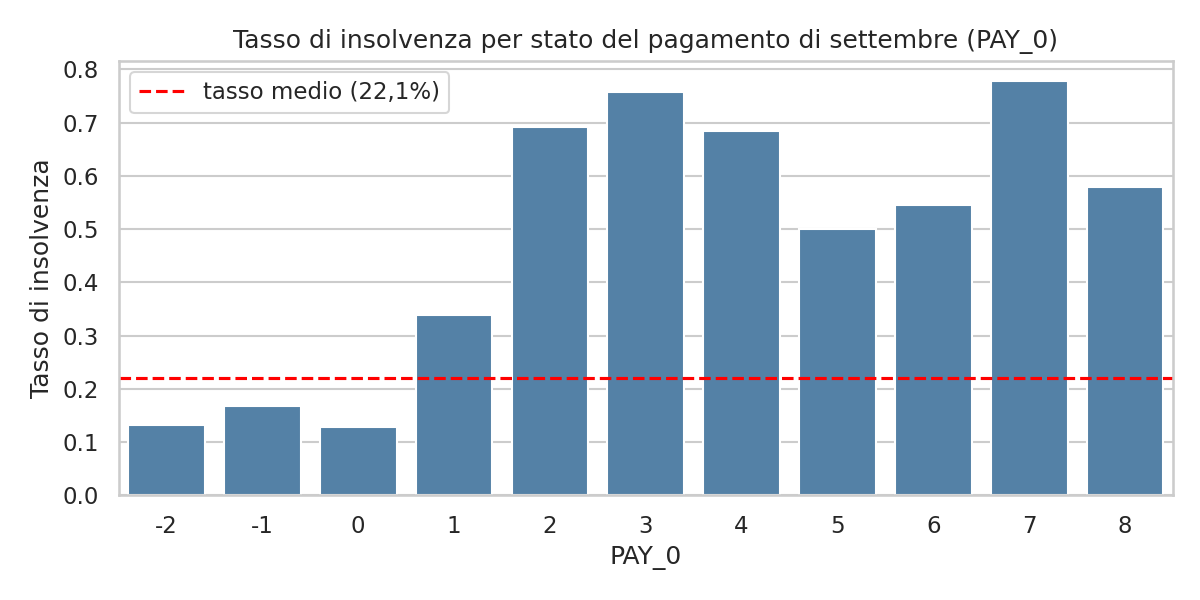
\includegraphics[width=0.85\textwidth]{images/barplot_pay0.png}
\caption{Tasso di insolvenza in funzione dello stato del pagamento di settembre (\texttt{PAY\_0}). La linea tratteggiata indica il tasso medio del campione (22,1\%).}
\label{fig:pay0}
\end{figure}

\begin{figure}[H]
\centering
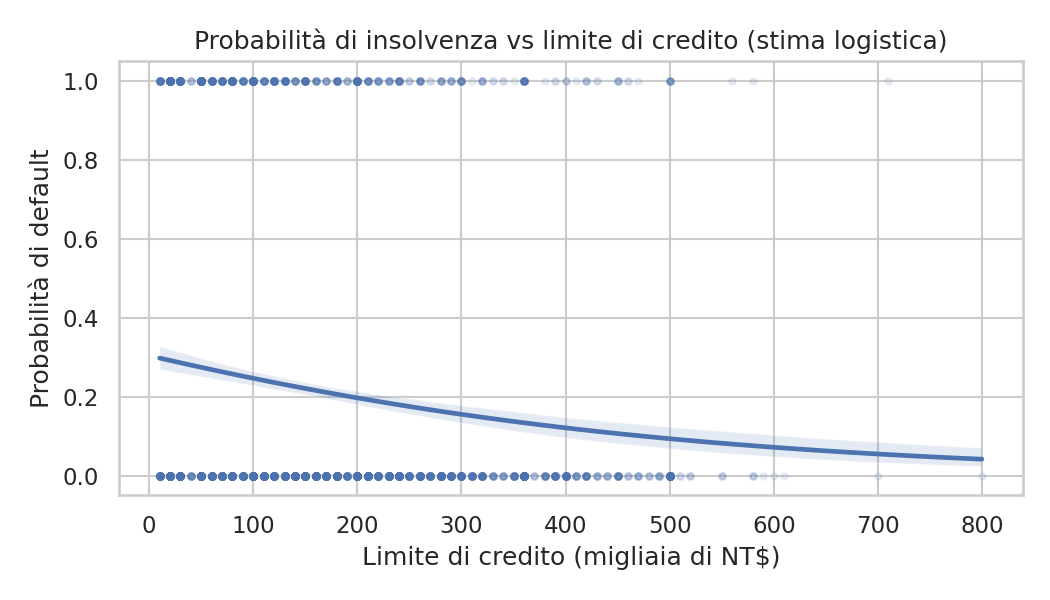
\includegraphics[width=0.7\textwidth]{images/regplot_limit_bal.png}
\caption{Probabilit\`a stimata di insolvenza in funzione del limite di credito (stima logistica univariata su un campione di 3.000 clienti). La probabilit\`a decresce in modo monotono senza mai avvicinarsi a 1: \texttt{LIMIT\_BAL}, da solo, \`e un predittore debole.}
\label{fig:regplot}
\end{figure}

\subsection{Preparazione dei dati}

Le variabili categoriche nominali (\texttt{SEX}, \texttt{EDUCATION}, \texttt{MARRIAGE}) sono state convertite in variabili dummy (one-hot encoding), per non imporre un ordinamento fittizio; le \texttt{PAY\_*}, ordinali, sono state mantenute numeriche. Il dataset \`e stato diviso in training (70\%, 21.000 clienti) e test set (30\%, 9.000 clienti) in modo \emph{stratificato}, preservando in entrambe le parti la quota di insolventi. Tutte le feature sono state standardizzate ($z = (x - \mu)/\sigma$) stimando $\mu$ e $\sigma$ sul solo training set, per evitare \emph{data leakage}: la standardizzazione \`e indispensabile per il $k$-NN, basato sulle distanze, e innocua per gli altri modelli.

\subsection{Modelli}

Abbiamo confrontato un modello lineare e due non lineari, tutti implementati con \texttt{scikit-learn}~\cite{sklearn} e con seme casuale fissato per la riproducibilit\`a.

La \textbf{regressione logistica} stima la probabilit\`a di insolvenza tramite la funzione sigmoide applicata a una combinazione lineare delle feature:
\begin{equation}
P(y = 1 \mid \mathbf{x}) = \frac{1}{1 + e^{-(\beta_0 + \beta_1 x_1 + \dots + \beta_p x_p)}},
\label{eq:logistic}
\end{equation}
e classifica come insolventi i clienti con probabilit\`a prevista superiore a 0,5. \`E il modello pi\`u interpretabile: il segno e la grandezza dei coefficienti $\beta_j$ indicano direzione e forza dell'effetto di ciascuna feature.

Il \textbf{$k$-Nearest Neighbors} classifica ogni cliente in base alla classe pi\`u frequente fra i $k$ esempi di training pi\`u vicini nello spazio standardizzato delle feature. Abbiamo confrontato $k \in \{5, 15, 25, 51\}$: valori piccoli producono modelli instabili, valori grandi appiattiscono le previsioni verso la classe maggioritaria; abbiamo scelto $k = 25$ come compromesso.

La \textbf{Random Forest} aggrega le previsioni di 100 alberi di decisione, ciascuno addestrato su un campione bootstrap dei dati e su sottoinsiemi casuali delle feature. \`E in grado di catturare relazioni non lineari e interazioni (come il brusco salto di rischio per \texttt{PAY\_0} $\geq 2$) e fornisce una misura di importanza delle feature. La scelta di 100 alberi \`e motivata da un esperimento dedicato (Sezione~\ref{sec:robustezza}).

\subsection{Metriche di valutazione}

Per ogni modello riportiamo accuracy, confusion matrix e, per la classe insolvente, precision, recall e F1-score, definito come media armonica:
\begin{equation}
F_1 = 2 \cdot \frac{\mathrm{precision} \cdot \mathrm{recall}}{\mathrm{precision} + \mathrm{recall}}.
\label{eq:f1}
\end{equation}

\section{Risultati}

La Tabella~\ref{tab:risultati} riassume le prestazioni dei tre modelli sul test set; la Figura~\ref{fig:cm} mostra le confusion matrix.

\begin{table}[H]
\centering
\caption{Prestazioni dei modelli sul test set (9.000 clienti). Precision, recall e F1 sono riferiti alla classe ``insolvente''. Baseline (classe maggioritaria): accuracy 0,779.}
\label{tab:risultati}
\begin{tabular}{lcccc}
\toprule
\textbf{Modello} & \textbf{Accuracy} & \textbf{Precision} & \textbf{Recall} & \textbf{F1} \\
\midrule
Regressione logistica & 0,809 & 0,698 & 0,240 & 0,357 \\
$k$-NN ($k=25$)       & 0,809 & 0,647 & 0,297 & 0,407 \\
Random Forest         & \textbf{0,813} & 0,636 & \textbf{0,366} & \textbf{0,464} \\
\bottomrule
\end{tabular}
\end{table}

\begin{figure}[H]
\centering
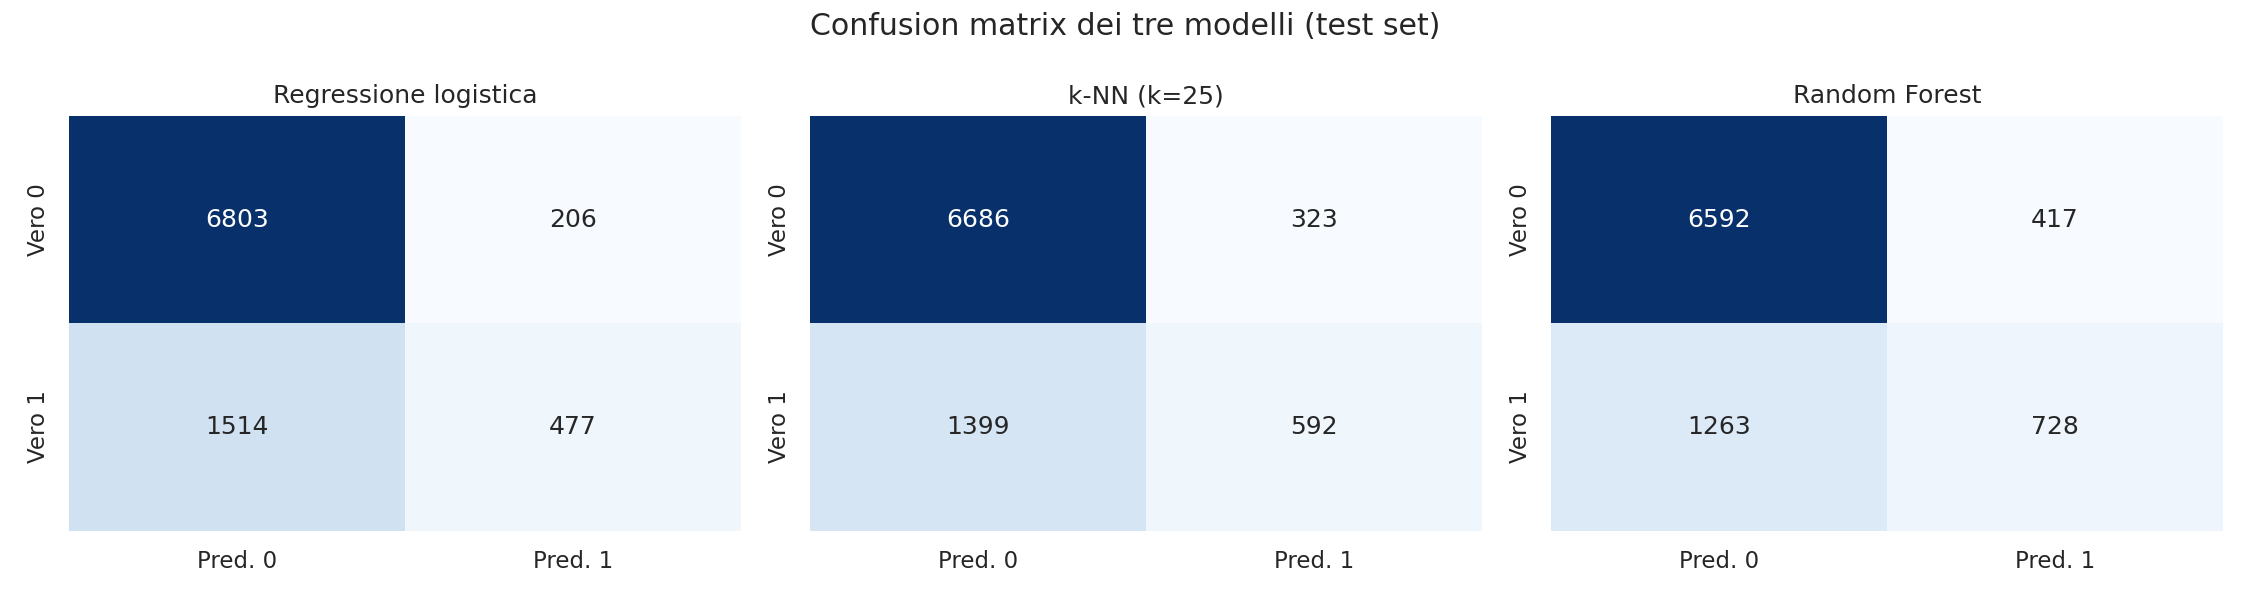
\includegraphics[width=\textwidth]{images/confusion_matrices.png}
\caption{Confusion matrix dei tre modelli sul test set.}
\label{fig:cm}
\end{figure}

Tutti i modelli superano la baseline, ma di poco in termini di accuracy (0,809--0,813): con classi sbilanciate il confronto significativo avviene sulla classe minoritaria. Qui emergono differenze sostanziali: la regressione logistica ha la precision pi\`u alta (0,698) ma individua meno di un insolvente su quattro (recall 0,240); il $k$-NN migliora leggermente il recall a scapito della precision; la Random Forest offre il compromesso migliore, con il recall (0,366) e l'F1 (0,464) pi\`u alti.

L'analisi dell'importanza delle feature della Random Forest (Figura~\ref{fig:fi}) conferma quanto osservato nell'analisi esplorativa: \texttt{PAY\_0} \`e di gran lunga la variabile pi\`u importante, seguita dalle altre variabili di ritardo e dagli importi; le variabili demografiche contano poco. Coerentemente, nella regressione logistica il coefficiente positivo pi\`u forte \`e quello di \texttt{PAY\_0} ($\beta \approx 0{,}65$ sulle feature standardizzate), mentre limite di credito e importi pagati di recente hanno segno negativo (riducono il rischio previsto).

\begin{figure}[H]
\centering
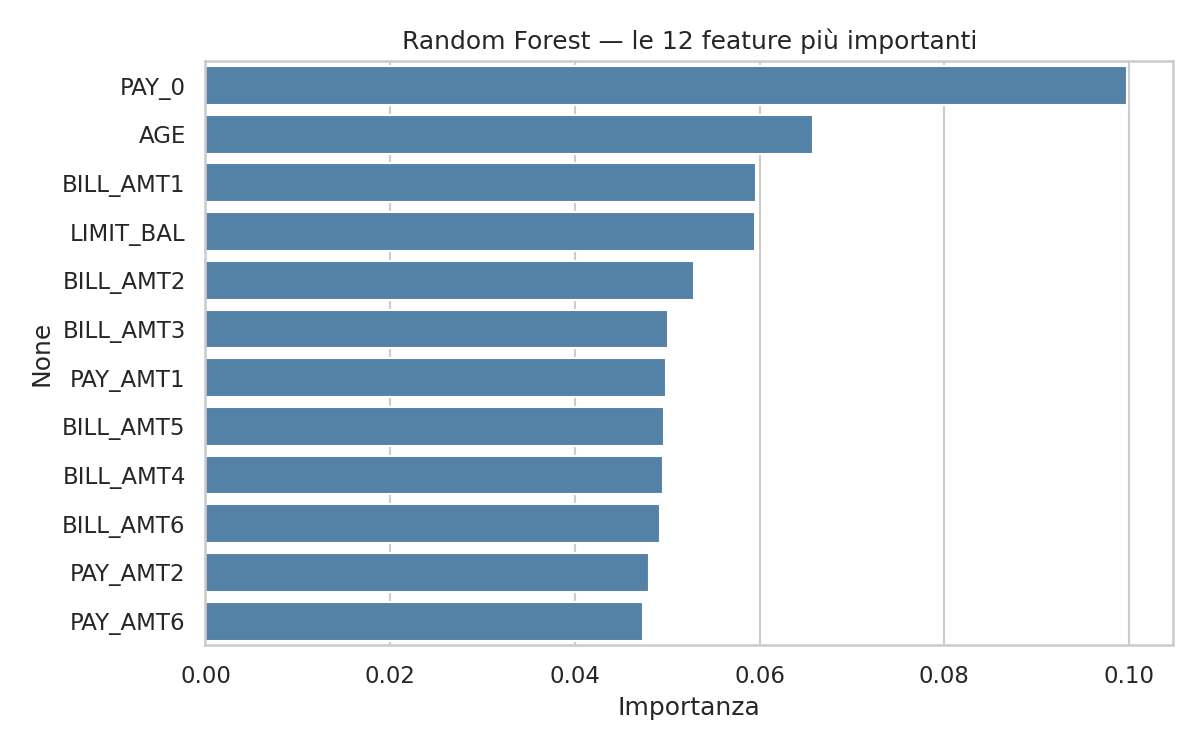
\includegraphics[width=0.8\textwidth]{images/feature_importance_rf.png}
\caption{Le dodici feature pi\`u importanti secondo la Random Forest.}
\label{fig:fi}
\end{figure}

\subsection{Esperimenti di robustezza}
\label{sec:robustezza}

Per verificare quanto i risultati dipendano dalle principali scelte di modellazione abbiamo condotto tre esperimenti.

\paragraph{Soglia di decisione della regressione logistica.} In un problema sbilanciato in cui i falsi negativi costano pi\`u dei falsi positivi, la soglia standard di 0,5 non \`e necessariamente adeguata. Abbiamo quindi valutato la regressione logistica al variare della soglia (Tabella~\ref{tab:soglie}): abbassandola da 0,5 a 0,3 il recall quasi raddoppia (da 0,240 a 0,456) e l'F1 sale a 0,503, superando la Random Forest a soglia standard (0,464), al prezzo di una precision che scende a 0,562; sotto 0,25 il compromesso peggiora rapidamente. Due limiti metodologici vanno dichiarati: la soglia \`e stata esplorata direttamente sul test set (rigorosamente andrebbe ottimizzata su un validation set separato) e il confronto non \`e del tutto equo, perch\'e anche agli altri modelli si potrebbe applicare una soglia ottimizzata. L'indicazione generale resta per\`o valida: \textbf{in questo problema la calibrazione della soglia incide sui risultati pi\`u della scelta dell'algoritmo}.

\begin{table}[H]
\centering
\caption{Regressione logistica al variare della soglia di decisione (test set). Precision, recall e F1 riferiti alla classe ``insolvente''.}
\label{tab:soglie}
\begin{tabular}{ccccc}
\toprule
\textbf{Soglia} & \textbf{Accuracy} & \textbf{Precision} & \textbf{Recall} & \textbf{F1} \\
\midrule
0,50 & 0,809 & 0,698 & 0,240 & 0,357 \\
0,40 & 0,812 & 0,630 & 0,370 & 0,466 \\
0,30 & 0,801 & 0,562 & 0,456 & \textbf{0,503} \\
0,25 & 0,752 & 0,452 & 0,560 & 0,500 \\
0,20 & 0,610 & 0,323 & 0,697 & 0,442 \\
\bottomrule
\end{tabular}
\end{table}

\paragraph{Numero di alberi della Random Forest.} Al variare di \texttt{n\_estimators} $\in \{10, 50, 100, 200, 500\}$ le metriche si stabilizzano gi\`a a partire da 50 alberi (F1 fra 0,459 e 0,467, differenze trascurabili), mentre il tempo di addestramento cresce linearmente, di circa dieci volte fra 50 e 500 alberi. Il parametro non \`e quindi critico per la qualit\`a delle previsioni: abbiamo adottato 100 alberi come miglior rapporto fra prestazioni e costo computazionale.

\paragraph{Proporzione dello split.} Ripetendo l'intera pipeline con split 80/20 anzich\'e 70/30 i risultati non cambiano in modo rilevante (scostamenti entro circa $\pm 0{,}02$ su tutte le metriche): con 30.000 osservazioni entrambi i training set sono gi\`a abbondanti, e ci\`o che cambia \`e soprattutto la rumorosit\`a della valutazione sul test set pi\`u piccolo. La proporzione dello split, entro valori ragionevoli, non \`e la leva su cui agire per migliorare i modelli.

\section{Discussione}

\paragraph{Interpretazione degli errori.} In ambito creditizio i falsi negativi (insolventi non individuati, con perdita del credito) sono tipicamente pi\`u costosi dei falsi positivi (clienti affidabili segnalati a torto). Con recall fra 0,24 e 0,37 alla soglia standard, tutti i modelli lasciano passare la maggioranza degli insolventi: l'esperimento sulla soglia mostra che gi\`a un semplice abbassamento a 0,3 riequilibra sensibilmente il compromesso; in un'applicazione reale la soglia andrebbe scelta in base ai costi effettivi dei due tipi di errore, eventualmente insieme a tecniche per dati sbilanciati (pesi di classe, ricampionamento).

\paragraph{Confronto fra i modelli.} La regressione logistica resta preziosa per interpretabilit\`a e costo computazionale minimo, ma il confine lineare non cattura il salto di rischio non lineare legato ai ritardi. Il $k$-NN non offre interpretabilit\`a e ha predizione lenta (deve calcolare le distanze da tutti i 21.000 esempi di training). La Random Forest \`e il modello pi\`u efficace a soglia standard e la feature importance ne mitiga la minore interpretabilit\`a, pur con un limite noto: la misura tende a sopravvalutare le variabili continue con molti valori distinti.

\paragraph{Limiti dell'analisi.} I principali limiti sono tre: (i) il recall modesto sulla classe minoritaria, legato allo sbilanciamento, che abbiamo mitigato esplorando la soglia di decisione ma senza tecniche di ricampionamento, per attenerci agli strumenti del corso; (ii) l'ambiguit\`a dei codici non documentati nelle variabili \texttt{PAY\_*}, per i quali abbiamo adottato un'interpretazione ragionevole ma non verificabile; (iii) la multicollinearit\`a fra le \texttt{BILL\_AMT}, che rende inaffidabili i coefficienti individuali di queste variabili nella regressione logistica.

\section{Conclusioni}

Abbiamo sviluppato un'analisi completa del dataset Credit Card Default: dalla comprensione critica dei dati (sbilanciamento, codici non documentati, ridondanza) al confronto fra tre modelli di classificazione, fino alla verifica di robustezza dei risultati. Il risultato principale \`e che il comportamento di pagamento recente --- in particolare \texttt{PAY\_0} --- domina la previsione dell'insolvenza, mentre le caratteristiche demografiche sono quasi irrilevanti. A soglia standard la Random Forest \`e il modello migliore (accuracy 0,813; F1 0,464 sulla classe insolvente), ma l'esperimento sulla soglia mostra che la calibrazione della soglia di decisione incide pi\`u della scelta dell'algoritmo: con soglia 0,3 la regressione logistica raggiunge F1 0,503. I risultati sono robusti rispetto alle scelte non critiche (proporzione dello split e numero di alberi): i margini di miglioramento stanno nella gestione dello sbilanciamento. Sviluppi futuri naturali includono pesi di classe o ricampionamento, l'ottimizzazione della soglia su un validation set separato e il feature engineering (ad esempio il rapporto fra importo pagato e fatturato).

\nocite{uci}
\bibliographystyle{unsrt}
\bibliography{bibliografia}

\end{document}
